\documentclass[svgnames,11pt]{beamer}
\input{/home/tof/Documents/Cozy/latex-include/preambule_commun.tex}
\input{/home/tof/Documents/Cozy/latex-include/preambule_beamer.tex}
%\usepackage{pgfpages} \setbeameroption{show notes on second screen=left}
\author[]{Formation 2022-2023}
\title{Construire un projet}
\date{\framebox{\textbf{NSI}}}
%\logo{}
%\institute{Formation NSI}

\begin{document}
\begin{frame}
    \titlepage
\end{frame}
\begin{frame}
    \frametitle{}

    \begin{center}
        \centering
        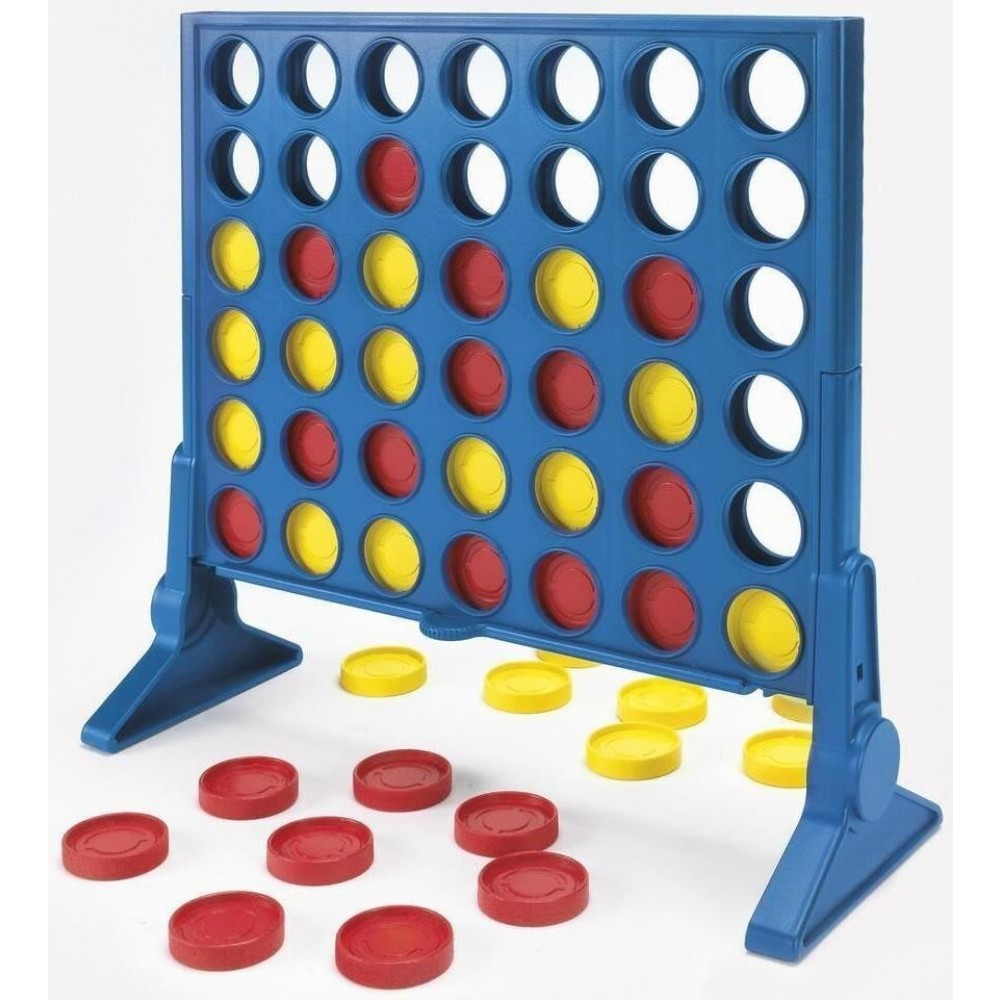
\includegraphics[width=8cm]{ressources/puissance4.jpg}
        \captionof{figure}{\centering Construire un premier projet avec les élèves.
        }
        \label{IMG}
    \end{center}

\end{frame}
\begin{frame}
    \frametitle{}

    Conditions:
    \begin{itemize}
        \item Chapitres déjà étudiés:
              \begin{itemize}
                  \item constructions élémentaires (affectation, condition, boucle, fonction)
                  \item tableaux
              \end{itemize}
        \item Projet de première.
        \item Premier projet.
    \end{itemize}

\end{frame}
\begin{frame}
    \frametitle{}

    \begin{framed}
        \centering Comment construire un projet?
    \end{framed}

\end{frame}
\section{Cycle de vie d'un projet}
\begin{frame}
    \frametitle{Cycle de vie d'un projet}

    \begin{center}
        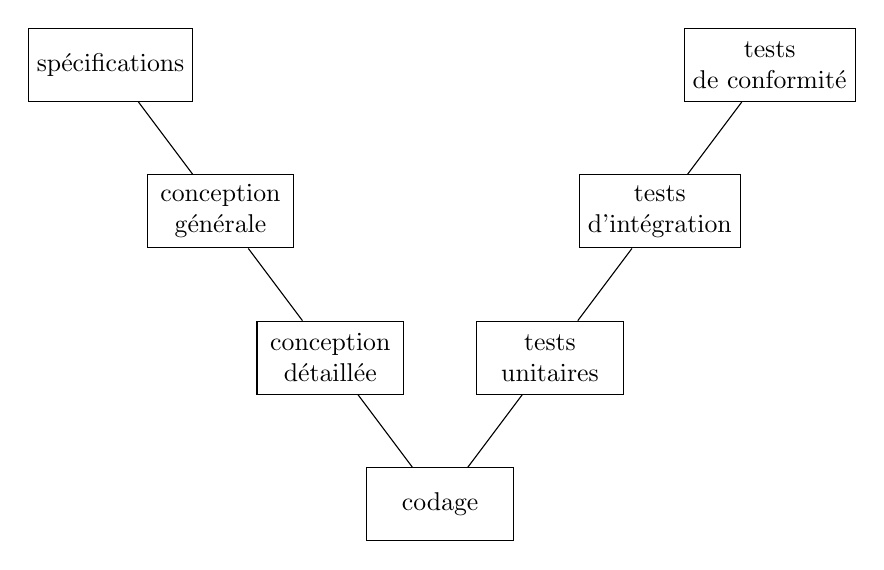
\begin{tikzpicture}[every text node part/.style={align=center}, scale=0.93,transform shape]
            \node[draw, minimum width=2cm, minimum height=1cm] (1) at(-4.5,6) {spécifications};
            \node[draw, minimum width=2cm, minimum height=1cm] (2) at(-3,4) {conception\\ générale};
            \node[draw, minimum width=2cm, minimum height=1cm] (3) at(-1.5,2) {conception\\ détaillée};
            \node[draw, minimum width=2cm, minimum height=1cm] (4) at(0,0) {codage};
            \node[draw, minimum width=2cm, minimum height=1cm] (5) at(1.5,2) {tests\\unitaires};
            \node[draw, minimum width=2cm, minimum height=1cm] (6) at(3,4) {tests\\d'intégration};
            \node[draw, minimum width=2cm, minimum height=1cm] (7) at(4.5,6) {tests\\de conformité};

            \draw (1) -- (2);
            \draw (2) -- (3);
            \draw (3) -- (4);
            \draw (4) -- (5);
            \draw (5) -- (6);
            \draw (6) -- (7);

        \end{tikzpicture}
    \end{center}

\end{frame}
\begin{frame}
    \frametitle{}

    \begin{center}
        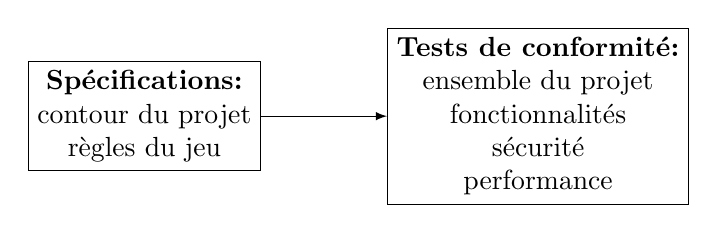
\begin{tikzpicture}[every text node part/.style={align=center}]
            \node[draw] (1) at(0,0) {\textbf{Spécifications:}\\contour du projet\\règles du jeu};
            \node[draw] (2) at (5,0) {\textbf{Tests de conformité:}\\ensemble du projet\\fonctionnalités\\sécurité\\performance};
            \draw[->,>=latex] (1) -- (2);
        \end{tikzpicture}
    \end{center}
    Exemple: Respect des règles du jeu
\end{frame}
\begin{frame}
    \frametitle{}

    \begin{center}
        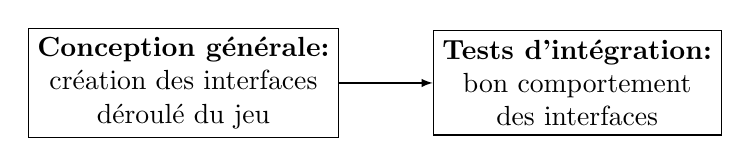
\begin{tikzpicture}[every text node part/.style={align=center}]
            \node[draw] (1) at(0,0) {\textbf{Conception générale:}\\création des interfaces\\déroulé du jeu};
            \node[draw] (2) at (5,0) {\textbf{Tests d'intégration:}\\bon comportement\\des interfaces};
            \draw[->,>=latex] (1) -- (2);
        \end{tikzpicture}
    \end{center}
    Exemple: Respect des différentes séquences du jeu (positionnement graphique du jeton\dots)
\end{frame}
\begin{frame}
    \frametitle{}

    \begin{center}
        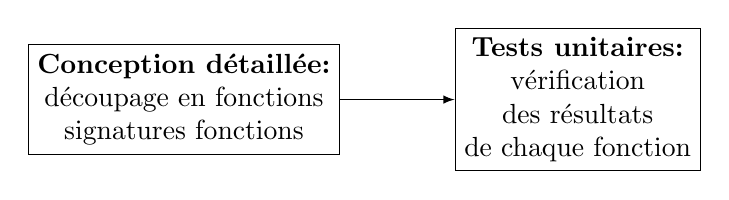
\begin{tikzpicture}[every text node part/.style={align=center}]
            \node[draw] (1) at(0,0) {\textbf{Conception détaillée:}\\découpage en fonctions\\signatures fonctions};
            \node[draw] (2) at (5,0) {\textbf{Tests unitaires:}\\vérification\\des résultats\\de chaque fonction};
            \draw[->,>=latex] (1) -- (2);
        \end{tikzpicture}
    \end{center}
    Exemple: Vérification de chaque fonction de calcul du gagnant (vertical, horizontal)
\end{frame}
\section{Puissance 4}
\subsection{Avec les élèves}
\begin{frame}
    \frametitle{Puissance 4 - Avec les élèves}

    \begin{itemize}
        \item <1->Premier projet de la classe de première.
        \item <2->Notions déjà abordées:
        \begin{itemize}
            \item constructions élémentaires,
            \item fonctions,
            \item types construits.
        \end{itemize}
        \item <3->Présentation de la construction de projet à travers un exemple détaillé.
    \end{itemize}

\end{frame}
\subsection{Spécifications}
\begin{frame}
    \frametitle{Spécifications}

    \begin{aretenir}[Rôle]
    Définir les règles du jeu.
    \end{aretenir}

\end{frame}
\begin{frame}

    \begin{itemize}
        \item une grille de 7 colonnes et 6 lignes,
        \item 2 joueurs en alternance (rouge et jaune),
        \item gagnant: 4 pions horizontaux, verticaux ou en diagonale.
    \end{itemize}

\end{frame}
\subsection{Conception générale}
\begin{frame}
    \frametitle{Conception générale}

    \begin{aretenir}[Rôle]
    Construire l'algorithme général du déroulé d'une partie.
    \end{aretenir}

\end{frame}
\begin{frame}

    \textbf{Initialiser} la grille\\
    Tant qu'il n'y a \textbf{pas de gagnant}:
    \begin{itemize}
        \item \textbf{Choisir} le joueur suivant.
        \item \textbf{Demander la colonne} choisie.
        \item \textbf{Vérifier} que la colonne n'est pas \textbf{pleine}.
        \item \textbf{Placer} le jeton en le \emph{laissant tomber} dans la colonne.
        \item \textbf{Afficher} la grille.
    \end{itemize}
    Partie terminée: \textbf{afficher} le gagnant.
\end{frame}
\subsection{Conception détaillée}
\begin{frame}
    \frametitle{Conception détaillée}

    \begin{aretenir}[Rôle]
    Spécifier le rôle et la signature de chaque fonction.
    \end{aretenir}

\end{frame}

\begin{frame}

    {\Large \textbf{\texttt{initialiser\_grille}}}
    \begin{itemize}
        \item rôle: construire la grille du jeu
        \item paramètres:
        \begin{itemize}
            \item nb\_col: entier
            \item nb\_lig: entier
        \end{itemize}
        \item renvoi: tableau de tableaux
    \end{itemize}

\end{frame}
\begin{frame}

    {\Large \textbf{\texttt{choisir\_colonne}}}
    \begin{itemize}
        \item rôle: demande la colonne où poser le jeton
        \item paramètres: aucun
        \item renvoi: la colonne choisie
    \end{itemize}

\end{frame}
\begin{frame}

    {\Large \textbf{\texttt{est\_remplie}}}
    \begin{itemize}
        \item rôle: vérifie si la colonne est remplie jusqu'en haut
        \item paramètres:
        \begin{itemize}
            \item grille: tableau
            \item colonne: entier
        \end{itemize}
        \item renvoi: booléen, vrai si la colonne est remplie
    \end{itemize}

\end{frame}
\begin{frame}

    {\Large \textbf{\texttt{placer\_jeton}}}
    \begin{itemize}
        \item rôle: place le jeton dans la grille
        \item paramètres:
        \begin{itemize}
            \item grille: tableau
            \item colonne: entier
            \item joueur: entier
        \end{itemize}
        \item renvoi: entier, la ligne où le jeton est placé
    \end{itemize}

\end{frame}
\begin{frame}

    {\Large \textbf{\texttt{verifier\_gagnant}}}
    \begin{itemize}
        \item rôle: vérifie si la partie est terminée 
        \item paramètres:
        \begin{itemize}
            \item grille: tableau
            \item joueur: entier
            \item ligne: entier
            \item colonne: entier
        \end{itemize}
        \item renvoi: booléen, vrai si le joueur a gagné
    \end{itemize}

\end{frame}
\begin{frame}

    {\Large \textbf{\texttt{dessiner\_grille}}}
    \begin{itemize}
        \item rôle: afficher la grille remplie
        \item paramètres:
        \begin{itemize}
            \item grille: tableau
        \end{itemize}
        \item renvoi: rien
    \end{itemize}

\end{frame}
\begin{frame}

    {\Large \textbf{\texttt{afficher\_gagnant}}}
    \begin{itemize}
        \item rôle: afficher le nom du gagnant 
        \item paramètres:
        \begin{itemize}
            \item joueur: entier
        \end{itemize}
        \item renvoi: rien
    \end{itemize}

\end{frame}
\begin{frame}
    \frametitle{}

\begin{aretenir}[Observation]
Il sera peut-être nécessaire d'écrire d'autres fonctions pour exécuter certaines tâches \emph{internes}:
\begin{itemize}
    \item \textbf{\texttt{verifier\_horizontal}}
    \item \textbf{\texttt{verifier\_vertical}}
    \item \textbf{\texttt{verifier\_diagonal}}
\end{itemize}
\end{aretenir}
\end{frame}
\subsection{Fourni aux élèves}
\begin{frame}
    \frametitle{Fourni aux élèves}

    Fournir le programme avec:
        \begin{itemize}
            \item le fichier de l'algorithme principal,
            \item toutes les signatures des fonctions,
            \item quelques fonctions non complétées.
        \end{itemize}

\end{frame}
\section{Lancement du projet}
\begin{frame}
    \frametitle{Lancement du projet}
\begin{itemize}
    \item <1->Choix du projet parmi:
    \begin{itemize}
        \item Morpion,
        \item ToutÉteint,
        \item Démineur (simplifié).
    \end{itemize}
    \item <2->Respect des étapes de conception
\end{itemize}
    

\end{frame}
\end{document}